%!TEX root = ./HW3.tex

\section{Grid World}
For grid world, two different types of learners are tested.  The first only estimates the expected reward of actions.  The second estimates the rewards based on state action pairs.  The performance of the state action pair is better.

\subsection{Problem Description}
In Grid World, the agent is spawned at a random location in the world.  The goal is a location on the map.  Every location that is not the goal gives a reward of -1 and the goal gives a reward of 100.  The length of an episode is 100 steps.  At the end of an episode, the agent is randomly spawned on the map.

\subsection{Results}
The learning progression is shown in Figure \ref{fig:GridLearn}.  The Q-Learning agent performs better than the Action Value agent.  An example trajector after training is completed is shown in Figure \ref{fig:GridQTraj} and Figure \ref{fig:GridAVTraj}.  In both situations, the episode length is 20 steps.  A random action is choosen randomly 20\% of the time.  The learning rate is 0.2, and the agents were stopped after 10,000 iterations.  However, convergence occurs within the first hundred iterations.  For both scenarios, ten trials were conducted with results shown including results from all ten trial runs.

\subsection{Analysis}
Action Value learning basically just walks around randomly.  Although moving down and the right seems to be the best move if the agent does not know where it is relative to the reward, the agent does not learn this.  This may be because the sparseness of the reward is not enough to overcome all of the small negative rewards.  The result is a random walk through the space, often staying in the same spot.  This is shown by the example trajectories in Figure \ref{fig:GridAVTraj}.  All of the action values are almost -1 which corresponds to the reward for all squares that do not hold the reward.  

Q learning performs much better.  The trade off is that significantly more information must be stored compared to the Action Value learner.  State action pairs are saved which requires an array 50 times larger than the action value table.  However, the Q-value agent is able to navigate to the goal optimally because of associating state actions with rewards.  This requires more iterations to converge, but allows the agent to understand the layout of the rewards as well as the best actions to achieve that reward.


\begin{figure}[h]
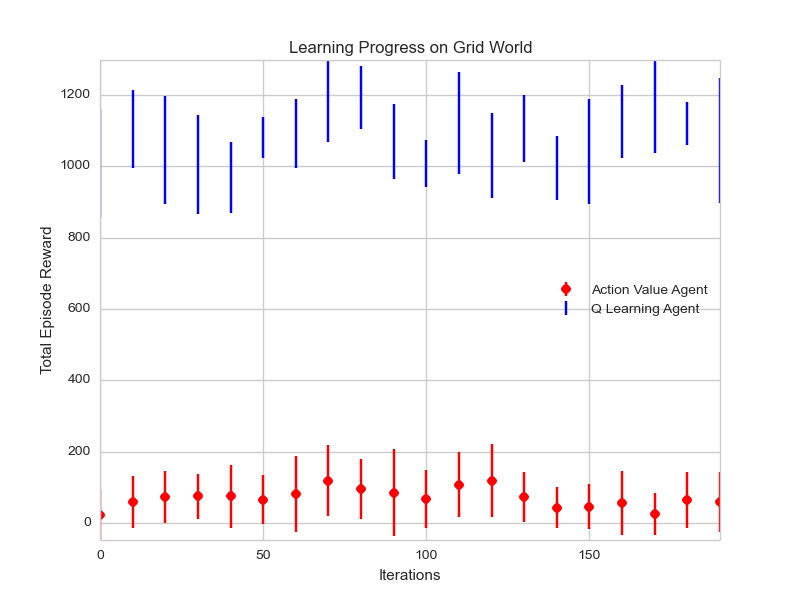
\includegraphics[width=1.0\linewidth]{GridWorldLearning.png}
\caption{Learning progress of both agents on grid world.  Q learning agent is able to improve over the course of training, where as the Action Value agent never improves significantly.}
\label{fig:GridLearn}
\end{figure}

\begin{figure}[h]
\centering
\begin{minipage}{0.45\textwidth}
\centering
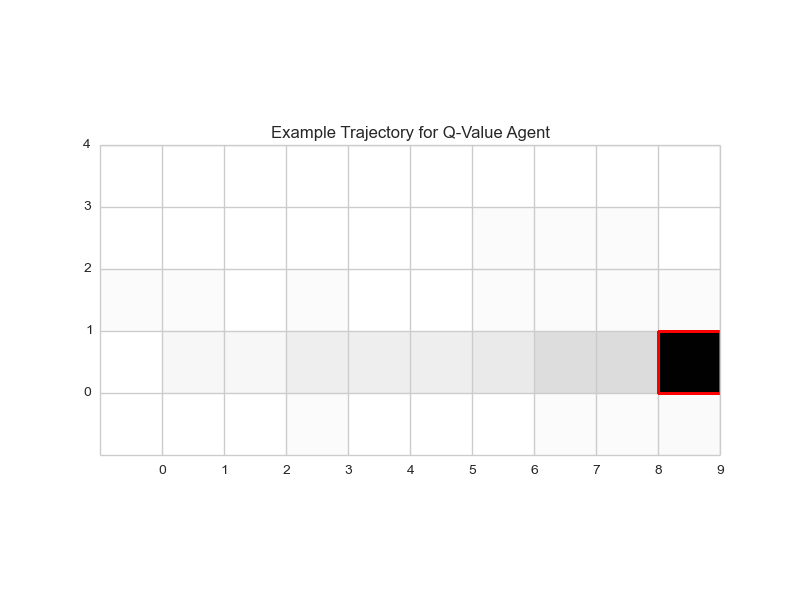
\includegraphics[width=0.98\linewidth]{GridWorldQTraj.png}
\caption{Converged Q-Value learning agent trajectories.  Darker colors indicate a square that is visited most often.  The test episodes only last 10 steps.  The agent learns the most direct route to the highest reward.}
\label{fig:GridQTraj}
\end{minipage}%
%
\hspace{0.08\textwidth}%
\begin{minipage}{0.45\textwidth}
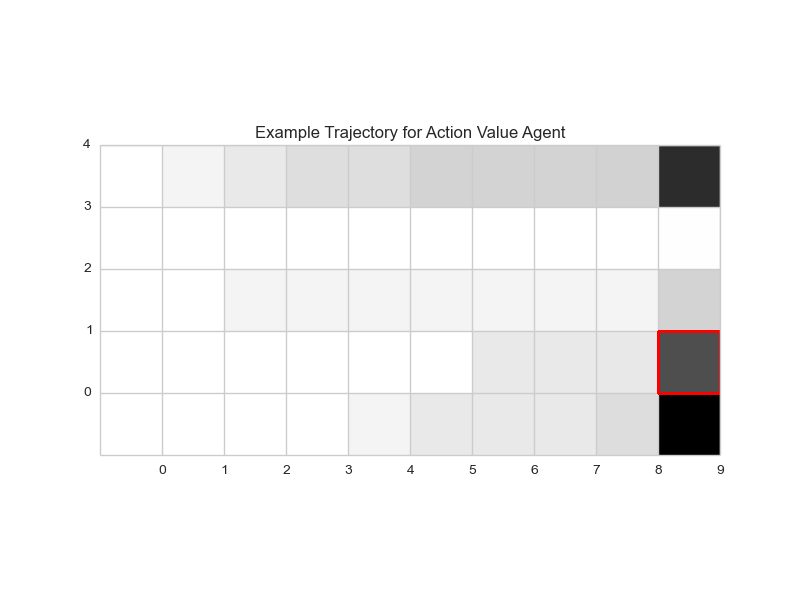
\includegraphics[width=\linewidth]{GridWorldAVTraj.png}
\caption{Converged Action Value learning agent trajectories.  Darker colors indicate a square that is visited most often.  The test episodes only last 10 steps.  The agent learns to go down and right regardless of location.}
\label{fig:GridAVTraj}
\end{minipage}
\end{figure}